\chapter{Design}
\label{chap:design}
This chapter describes design of the whole platform in details, however implementation specifics of some parts of the tool are described in the following chapter.  This chapter starts with an overview of the complete platform and follows by a simple use-case to give the reader idea how this tool is mean to be used. 

Spans and their format are described next followed by design of the native agent and instrumentation server. This chapter ends by describing the used Zipkin user interface and also JSON format in which the user interface accepts the data from the instrumentation server. 


\section{Overview}
This section gives high-level overview of the platform and shortly describes the basic parts and the relations between each part. Main purpose of this tool is to collect distributed traces. In order to achieve that, the thesis is based on the concept of Spans. Spans are used to denote some specific part of the communication between the communicating nodes and are the important elements for building the whole trace trees. Trace trees consists of several spans and represent the complete task or communication where a span inside the trace represents usually a few remote procedure calls between two neighboring nodes. The node initiating the trace creates so called parent span and new calls started within this span create new nested spans. Created spans can be processed using different span savers and can be send to the user interface using various data collectors. 

Spans are processed using Span Savers. Span savers are used to save spans in desired format on disk or on the network for further data collection and collected data are used for Spans visualizations in the user interface. The user interface receives the spans from the span savers or data collectors and present them to the user in a form of trace trees.

Definition of when a new span is to be created and when an existing span needs to be closed is done by a developer by extending the core instrumentation server library. The created instrumentation server is then used for instrumenting the classes of the original application at which information about spans needs to be preserved. In order to obtain the class files, the native agent runs  as part of the monitored application and sends the instrumentation server the desired classes. The native agent is the core part of the whole platform. It is attached to the monitored application and additionally to the instrumentation, it is used to obtain various low-level information from the application. 

The tool therefore consists of three main parts:
\begin{itemize}
	\item Native Agent
	\begin{itemize}
		\item Is used to obtain byte-code for the instrumentation
		\item Is used to actually apply the instrumented byte-code
	\end{itemize}
	\item Instrumentation Server
	\begin{itemize}
		\item Instruments the classes obtained from the native agent
		\item Is also a base library for custom application instrumentation server
		\item Can contain implementations of custom span savers
	\end{itemize}
	\item User Interface
\end{itemize}

\section{Example Use Case}
In order to have a better understanding how this platform can be used we provide simple example of client-server application as an use-case, so far without the code. Clients query the server and server provides them with the response. We would like to instrument the client and the server and monitor the communication between the client and the server.

Because client and the server are different applications, we need to create 2 different instrumentation servers and specify what is the method and a class which is required to be instrumented and what should happen in the instrumented code. In this case we just want to add custom annotations to recorded spans which are specific to the client-server communications.

The native agent has to be attached to both the client and the server prior it's start and the path to the instrumentation server jar needs to be set on both client and server to corresponding server. The default span sever is used in this case and the collected spans are send right to the Zipkin UI. The default endpoint for the user interface is used when not defined as an argument to the native agent.

We can see that the only part the user needs to worry about is the extension of the instrumentation server to specify the custom instrumentation points, otherwise the rest of the work is done automatically.

\section{Spans and Trace Trees}
\label{subsec:spans}
Span is the main concept used for capturing distributed traces. They are special classes which instances are injected to instrumented classes to keep track of the communication and the state between the nodes in the distributed application. Usually, the initiator creates so called parent span and new calls started within the span creates new nested spans. The only information required to be available in Span class is its id and parent span id and in order to be able to distinguish different spans, also unique trace id which is created during root span creation. 
As mentioned briefly in the previous section, spans are used to gather the information about the distributed calls or so called, distributed stack traces. Spans are defined as part of the Instrumentation server but since it's the most important concept in the thesis, we explain them in the separated section. 
Created spans are processes using different span savers and can be send to the user interface using various data collectors.
Spans has several mandatory and optional fields. The mandatory fields are trace id, id and parent id. Trace id represents one complete distributed call among all interacting nodes on the cluster. The field is attached automatically when a new root span is created. Root span is a first one which is created inside a trace. The root span does not have parent id field set up so the user interface backend can distinguish between regular spans and root spans. Parent if of a span is always id of span from which we received a request to perform some task. The span and its parent span can be located on the same node and on different nodes as well. The first can be useful in cases we would like to capture the communication between different threads on the same node in the same manner as the rest of cluster communication

Span have several additional fields which are set and are used in the Zipkin UI. Each span has also
\begin{itemize}
	\item \textbf{Timestamp} - when the span started
	\item \textbf{Duration} - how long the span lasted
	\item \textbf{Annotations} - annotations which are used to carry additional timing information about spans. For example time when span has been received on the receiver side or the time the span has been processed at the receiver side can be set using the annotations.
	\item \textbf{Binary annotations} - annotations which can be used to carry around application specific details. We can use these annotations to transfer information between communication nodes inside of Spans. For example one node can store number number of bytes sent during the request and the receiver can use this information to calculate overall number of bytes received from this particular node.
\end{itemize}

Each annotation has also endpoint information attached. This consist of:
\begin{itemize}
	\item \textbf{ip} - ip of node on which this event is recorded
	\item \textbf{port} - port on which the service which recorded the span is running
	\item \textbf{service name} - service name can be used to group different traces by names and can be later used to filter such traces in the user interface
\end{itemize}

The following sections contains information about how span are exported for external communication and also how spans are created using \texttt{TraceContext} and \texttt{TraceContextManager} classes.
\subsection{Span Savers}
The platform allows the user to create custom span savers which can be used to plug-in custom data collectors and custom user interface. Spans are internally represented in JSON format. The thesis contains support for working with JSON data and it is explained in more detail later in the  \hyperref[chap:implementation]{Implementation} chapter. In order to be able to send span data to corresponding user interface or just to save them on disk the spans can be processes using various span savers.

Each saver has to extend from abstract ancestor defining common methods for each span saver. Also in order to be able to use the saver automatically in the code, it has to have a constructor with single \texttt{String} argument accepting saver arguments.

SpanSaver abstract class has 2 abstract methods:
\begin{itemize}
	\item \texttt{saveSpan}. This method is used for saving span. Custom span saver implementaion may save the data on local disk or send over network. The destination is not limited.
	\item \texttt{parseAndSetArgs}. The instrumentation agent accepts also argument which contains arguments for the defined span saver. Each span saver is responsible for parsing the arguments.
\end{itemize}

Spans are processed asynchronously using executor service using the span savers. By default, the platform supports 2 simple span savers:
\begin{itemize}
	\item  \texttt{DirectZipkinSaver} - The default span saver sends asynchronously the collected span to the user interface right away without storing the data for disk to be collected by an external data collector. In this case the functionality the span saver and the data collector functionalities are handled by this single saver. This span saver should be used for demonstration purposes only since  it could overload the user interface or network when processing and sending high amount of collected spans in a short amount of time to the user interface as the UI is not prepared to store large amounts of data in the memory. 
	
	This saver accepts a single argument which is ip and port of the Zipkin UI service.
	\item  \texttt{JSONDiskSaver} - The second available span saver saves the collected data asynchronously on disk in the format known to Zipkin UI for future collection to the Zipkin user interface via custom data collector. Together with some well-known data collection agent, this is a preferred way of transferring spans from the application to the user interface in the production. This saver  accepts single argument which is a directory where collected spans are saved.
\end{itemize}


In order to be able to allow the flexibility to add new savers, we have register them in the META-INF directory of the generated JAR file. This ensures that the service loader can find all implementations of the \texttt{SpanSaver} abstract class. The reason why the classes needs to be discovered is explained in the following Native Agent section. To make the developer life easier we use the \textbf{AutoService}  library from \textit{https://github.com/google/auto/tree/master/service}. Instead of manually registering the implemented span savers into META-INF directory, we can annotate them with \texttt{AutoService} annotation with a single argument specifying the abstract parent. The library then takes care of registering the classes automatically so the human error is minimized.

\subsection{Trace Context}
Trace context is class used for storing the information about the current span and also for creating new and closing current spans. Trace context is always attached to a specific thread. This is done in order to allow multiple threads to have different computation state and therefore the platform is able to capture multiple distributed traces at the same time on the same node. Singleton instance of class \texttt{TraceContextManager} is used for attaching the threads to the trace contexts and vice-versa. It has a few methods allowing us to attach trace context to a specific thread and also to get trace context which is attached to a current thread.

Each trace represented by a trace context is uniquely identified by \texttt{Universally unique identifier (UUID)} of type 1 is created. The version 1 of UUID combines 48-bit MAC address of the current device with the current timestamp. This way it is ensured that 2 traces created at the same time on different nodes can't have the same identifier. The identifiers are created using a C++ library called sole (https://github.com/r-lyeh/sole) in the native agent and are made available to the Java code via a published native method.

The trace contact has method \texttt{openNestedSpan} and \texttt{closeCurrentSpan}. The first is used to create a new nested span and set the newly created span as the current one. Nested span is a span which sets its parent id to the current span. A root span is created in case when no current span exists. The second method is used to close the current span. Closing the span triggers the span saver attached to the span and moves one level higher in the span hierarchy to the previous current span.

\section{Native Agent}
The native agent is used for accessing the internal state of the monitored application and to instrument classes to allow us to attach the span and trace identifiers to classes transferred between the application nodes. 	The main task for the agent is to check weather a class is required to be instrumented and if yes, send the class for the instrumentation to the server and wait for the instrumented code.

The native agent consist of several parts. The most important parts are:
\begin{itemize}
	\item \textbf{Bytecode parsing module}. The classes in this module are used to parse the JVM bytecode in order to discover the classes dependencies for further instrumentation. Bytecode parsing is a technical task described in the following Implementation chapter.
	\item \textbf{InstrumentorAPI}. This class is provides several methods which are used to communicate with the instrumentor JVM. All the queries to the instrumentor are done via instance of this class.
	\item \textbf{AgentCallbacks}. All callbacks used in the native agent are defined in this namespace.
	\item \textbf{AgentArgs}.  This class contains all the logic required for argument parsing.
	\item \textbf{NativeMethodsHelper}. This class is used for registering native methods defined in C++. These methods can be later used from the Java code without worrying of the low-level implementation.
	\item \textbf{Utilities module}. This module contain several utility namespaces. The most important utility namespances are \textbf{AgentUtils} and \textbf{JavaUtils}. The first one is contains method for managing the JVMTI connection together with method for registering the JVMTI callbacks and events. The second one is used for easier work with Java objects in the native code via JNI. 
\end{itemize}

\subsection{Agent Initialization}
The agent is initialized via the same phases as described in the \hyperref[subsec:jvmti_init]{JVMTI Agent Initialization}  section of the \hyperref[chap:background]{Background} chapter. For the thesis purposes, we are interested in the following events: \texttt{VM Init}, \texttt{VM Start}, \texttt{VM Death}, \texttt{Class File load Hook}, \texttt{Class Prepare} and \texttt{Class Load} event. Callbacks are registered for all the mentioned events so we can react to them accordingly in the code.


As part of the initialization process the agent is responsible for either connecting to or starting a new instrumentation server. In case the native agent was started in the shared mode of the instrumentation server, the agent tries to connect to already existing server and is shared between all application's nodes. In the local instrumentation mode, the instrumentation server is started as a separated process and the connection is established with the server using the inter process communication. In this case, each application node has dedicated instrumentation server.

The callback registered for the \texttt{VM Init} event is is responsible for loading all additional classes from the instrumentation server as part of the initialization as well. The additional classes are for example \texttt{Span}, \texttt{TraceContext} or custom implementations of \texttt{SpanSaver} abstract class and have to be available to the monitored application since the instrumented code require them as dependencies. The native agent is designed as a code which users should not need to touch and define all application specific code in the instrumentation server extension. Therefore the instrumentation server is asked at the initialization phase for the list of all additional classes and they are sent to the native agent. The agent puts all the received classes on the application's class-path so they are available to the instrumented code.

\subsection{Instrumentation}
Code handling the instrumentation is part of the callback for the \texttt{Class File load Hook} event. The callback has the bytecode for the class which is being loaded on its input and allow as to pass a new instrumented bytecode as the output parameter. The process of instrumentation is described here however the technical details are described in the following chapter.

The process consist of several stages:
\begin{enumerate}
	
	\item Enter the critical section. It can happen that the class file load hook is triggered multiple times and in order to not confuse the instrumentation server, we have to lock before we start instrumentation of a class.
	\item Firstly, we check if the virtual machine is started since we don't need to instrument System classes at this moment.
	\item Attach JNI environment to the current thread. Since the JVMTI and JNI does not have automatic thread management, it's up us to take care of correct threading management.
	\item Discover the class-loader used for loading the class
	\item Parse the name of class being loaded. Even though the callback provides input parameter which should contain the name of loaded class, at some circumstances it can be set to \texttt{NULL} even though the class is correct. Instead of relying on this parameter, we parse the class name from the bytecode ourselves.
	\item Decide weather we should continue with the instrumentation. This check is based on the used class loader and name of the class being loaded. Classes loaded by the \texttt{Boostrap} classloader and in case of Sun JVM, from \texttt{sun.reflect.DelegatingClassloader} are not supposed to be instrumented. 
	The \texttt{Boostrap} is used to load system class and the second mentioned class-loader is used to load synthetic classes and in both cases, it's not desired to instrument classes loaded by these classloaders.
	There are also some ignored classes for which the instrumentation is not desired. Example of these classes are the classes loaded during initialization phase from the instrumentation server and the auxiliary classes generated by the Byte Buddy framework. Auxiliary classes are small helper classes Byte Buddy is using for example for accessing the super class of the currently instrumented class. Therefore we proceed to the instrumentation only If the class is not ignored and not loaded by ignored class loader.
	\item We ask the instrumentation server whether it already contains the loading class or not and also if the class should be instrumented. The agent does not know which classes are to be instrumented and it therefore needs to query the server. The other could be be to specify which classes should be instrumented as arguments to the native client but that would be hard to manage since it would be static list of classes and more complicated deployment for the end user as well. In this approach the developer can specify which classes can be instrumented on the instrumentation server using simple Byte Buddy API. 
	
	If the server does not contain the class, we send the class data to the instrumentation server, parse the class file for all the dependent classes and send all dependent classes to the instrumentation. This step is repeated throughout the dependency scan recurrently until the class does not have any other dependencies or until the dependency is already available on the server. All dependencies for the currently instrumented class have to be available on the server in order to perform the instrumentation.

	\item At this stage, the class is already on the instrumentation server and all dependencies for this class as well. Therefore, at this step we can proceed with the instrumentation itself and ask the server for the instrumented class.
	\item Exit the critical section.
\end{enumerate}	
Even though the class is not fully instrumented and the instrumented byte-code is available to the agent, the process is not completely done. The instrumentation library used at the instrumentation sever ( Byte Buddy) is using so called \texttt{Initializer} class to set up the interceptor field in the instrumented classes. It is a static field which references the instance of the class interceptor. This field is automatically set by Byte Buddy framework in most of the cases but since we are instrumenting on different JVM then where the code is actually running, we need to handle this case as well. In order to set this field by corresponding \texttt{Initializer} class we need to have both the initializer class and interceptor available on the agent. The instrumentation server sends the initializer class together with the instance of interceptor during the instrumentation of the class and the agent register the interceptor and initializers with the instrumented class for later since we need to wait for the class to be used for the first time to set the static field to a corresponding interceptor. The initializers are loaded during  \texttt{Class Prepare} event handling. This event is triggered when the class is prepared but no code has been execute so for. 

This callback for this event is also used to register the native methods for the class being loaded. By registering the native method to the class we make it available from Java programming language.

Several technical difficulties had to be dealt with during the development. For example, we need to properly handle cyclic dependencies when instrumenting the class. Also ensuring that the dependencies for the instrumented class are also instrumented in the correct order has been a significant challenge. The different attempts for the solution and the final solution is described in the following chapter since it's highly implementation specific.
\subsection{Instrumentation API}
The Instrumentation API is used to communicate with the instrumentation server. It provides low-level method for sending data in form of byte arrays or strings and the corresponding methods for receiving the data. On top of these method several methods is build to make the communication easier. The most important methods are:
\begin{itemize}
	\item \texttt{sendClassData} method sends byte code to the instrumentation server.
	\item \texttt{isClassOnInstrumentor} method checks weather the bytecode for the given class is already on the instrumentation server or not.
	\item \texttt{instrument} method triggers the instrumentation and returns the instrumented bytecode.
	\item \texttt{loadInitializersFor} method is for loading the initializers for specific class.
	\item \texttt{loadDependencies} method is used to load all dependent classes and upload them on the instrumentation server. The dependency is uploaded only in case it's not already available on the instrumentation server.
	\item \texttt{shouldContinue} method checks weather the class on its input is allowed to be instrumented.
	\item \texttt{loadPrepClasses} method loads all dependent classes in the agent initialization phase.
\end{itemize}

\subsection{Native Agent Arguments}
The native agent accepts several arguments which can be used to affect the agent behavior. In local instrumentation server mode several arguments affect also the sever started from the agent. Available arguments are:
\begin{itemize}
	\item \textbf{instrumentor\_server\_jar} - specifies the path to the instrumentation server jar. It is a mandatory argument in case the instrumentation server is supposed to run per each node of monitored application.
	\item \textbf{instrumentor\_server\_cp} - specifies the classpath for the instrumentation server. It can be used to add application specific classes on the server classpath which has the effect that the monitored application does not have to send the server these classes if they need to be instrumented or if some class to be instrumented depend on them.
	\item \textbf{instrumentor\_main\_class} - specifies the main entry point for the instrumentation server. It is a required argument in case of local instrumentation server mode.
	\item \textbf{connection\_str} - specifies the type of connection between native agent and the instrumentation server. It is a mandatory argument in shared instrumentation server mode in which case the value is in format \texttt{tcp://ip:port} where ip:port is address of the instrumentation server. Otherwise the agent and server communicates via inter-process communication and the argument can be set in format \texttt{ipc://identifier} where identifier specifies the name of pipe in case of Windows and name of the file used for IPC in case of Unix. However this value is set automatically at run-time if not explicitly specified as an argument.
	\item \textbf{log\_dir} - specifies the log directory for the agent and when running in local server mode, specifies the log directory for the server as well.
	\item \textbf{log\_level} - specifies the log level for the agent and when running in local server mode, specifies the log level for the server as well.
	\item \textbf{saver} - specifies the span saver type. The value can be either \texttt{directZipkin(ip:port)} where ip:port is address of the Zipkin UI interface or \texttt{disk(destination)} where destination sets the output directory for the captured spans. Custom span savers are supported as well. In that case the format of the value is a fully qualified name of the span saver with arguments in parenthesis, for example as \texttt{com.span.saver(arguments)}
	\item \textbf{config\_file} - specifies path to a configuration file containing agent configuration. It can contain all arguments mentioned above, each argument per 1 line of the configuration file.
\end{itemize}

\section{Instrumentation Server}
\label{sec:inst_server}

The instrumentation server also acts as the base library for the instrumentation for specific applications. Usually the user needs to have the code for instrumentation server available as a dependency and can use prepared method to define custom instrumentation points without touching the internals of the native agent.

The instrumentation server needs to deal with several technical problems. The main issue is that the classes which are about to be instrumented require all other dependent classes to be available as well. The other issue is for example instrumenting the classes with circular dependencies. The server also performs several optimizations to provide faster response to the agent such as caching the instrumented classes or minimizing the communication when possible. The technical aspects of the issues and the optimizations mentioned above are described in the following sections.


The instrumentation server is responsible as the name suggest for instrumenting the byte code. The native agent asks the server weather the class is required to be instrumented, the server then received the byte code, performs the instrumentation and sends the data back to the agent. It does not contain any application state and does not know about the distributed traces.

Instrumentation server is responsible the the code instrumentation in separated virtual machine then the application is running. In this section we cover several design aspects of the instrumentation server, leaving the implementation details on the following sections. As already mentioned, the server can run locally on each application node or it can be shared among all the application nodes. The core instrumentation on the server is handled by the Byte Buddy code manipulation framework.

The platform was designed to be configurable and deployment of instrumentation server is supported using two methods. The instrumentation server can be either on the network available to all the application nodes and can be shared by all applications. This has an advantage of caching the instrumented classes. So when any class is instrumented for the first time, the instrumentation is not performed for other nodes but the class is immediately sent. The disadvantage of this solution is higher latence between the agent and the instrumentation server since they are usually not on the same node. In this case the instrumentation server has to be manually started in advance. Architecture of this scenario is depicted on the diagram \ref{fig:shared_server}.
 
 \begin{figure}
 	\centering
 	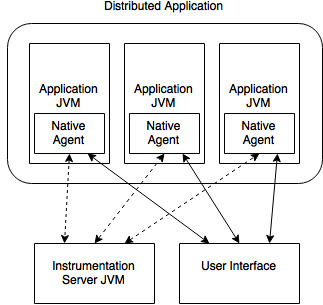
\includegraphics[scale=0.8]{shared_server.png}
 	\caption{Architecture with shared instrumentation server. The dotted lines represents the communication between instrumentation server and the agent whilst the regular lines represents data collection from the agent to the UI}
 	\label{fig:shared_server}
 \end{figure}
 
 The other deployment method is that the instrumentation server runs on each application node. This has the advantage of faster communication since we can use inter-process communication methods to communicate between monitored JVM and the instrumentation server. The disadvantage of this solution is that we have to instrument all classes on each node since there is no communication between the instrumentation servers. In this solution, the server is started automatically during the native agent initialization. Architecture of this scenario is depicted on the diagram \ref{fig:separated_server}.
 
 \begin{figure}
 	\centering
 	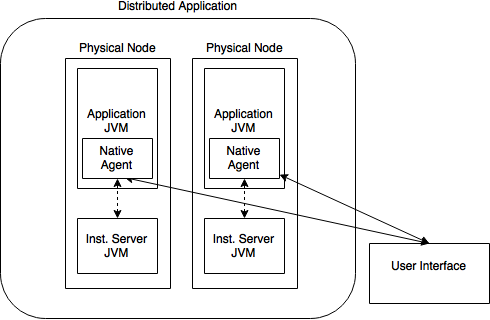
\includegraphics[scale=0.8]{separated_server.png}
 	\caption{Architecture with separated instrumentation server. The meaning of the lines is the same as on the diagram above.}
 	\label{fig:separated_server}
 \end{figure}


Except from the cached classes, the server does not contain any application state and it just reacts to the agent requests. It can accept four type of requests:
\begin{itemize}
	\item Request for code instrumentation.
	\item Request for storing byte code for a class on the server.
	\item Request for sending dependency classes needed by the agent
	\item Request to check whether the server contains specific class or not.
\end{itemize}
The server interacts in more ways with the agent, however they are just sub-parts of the communication initiated by one of these 4 request types.	

\subsection{Instrumentation}
The instrumentation of the class is triggered by the agent and it's done in 2 stages. The first stage informs the client whether the class is already on the instrumentation server or not. The second stage is the instrumentation itself. The first stage is initiated by the agent who asks the server whether the class is available on the server or not. The server performs this check in 3 phases:
\begin{enumerate}
	\item Check whether the instrumented bytecode for this class is available
	\item If not, check wether the original bytecode for this class is available
	\item If not, check if we can load the class using our context class loader. This handles the cases where the user builds the instrumentation server together with the application classes or adds the application classes on the instrumentation server classpath. 
\end{enumerate}

The server informs the client if it does not have the class, the agent sends the class and the server registers the received byte-code under the class name. The agent therefore does not have to send the class next time since it's already cached on the instrumentation server.
The second stage follows the first stage immediately the first one. If the server already contains the instrumented class in the cache, it sends it right away without instrumenting the class again. If the cache is empty, the class is instrumented and put into the cache.

The code instrumentation is handled by \texttt{CustomAgentBuilder }and \texttt{BaseAgentBuilder} classes.
The instrumentation server expects instance of \texttt{CustomAgentbuilder} on the input of its start method. This is abstract class containing single abstract method \texttt{createAgent(BaseAgentBuilder builder, String pathToGeneratedClasses)} where the builder is wrapper around the Byte Buddy \texttt{AgentBuilder} class which is used to define the class transformers.

The user needs to implement this method and specify on which classes and on which methods the instrumentation should happen. Since Byte Buddy is used for writing transformers and interceptors, please read more about Byte Buddy in the \hyperref[sec:byte_buddy]{Byte Buddy} section. The server provides several helper methods for creating the transformers and interceptors which are less verbose then the standard Byte Buddy approaches.

Each created transformer has to have associated some interceptor which defines the instrumented code. Each interceptor has to implement \texttt{Interceptor}  interface. This is required for the server to be able to discover all interceptors at run-time without the need for changing the internals of the sever. Each implementation of the interceptor needs to register itself in the META-INF directory of the generated jar in a same way as it the span savers mentioned in the previous section. Custom service loader is then used to locate all classes implementing the \texttt{Interceptor} interface.

Even though Byte Buddy takes care about the instrumentation, the \texttt{BaseAgentBuilder} class is internally properly configured so the instrumentation happens exactly as desired. The class implements for 4 byte buddy listeners used for informing us about the instrumentation progress and allow us to react on the process of the instrumentation. The listeners are:
\begin{itemize}
	\item \texttt{onTransformation} listener is called immediately before the class is instrumented. Our implementation of the listener also sends the agent all auxiliary classes required by the instrumented class and the initializers used for setting the static interceptor field on the instrumented class.
	\item \texttt{onIgnored} listener is called when the class is not instrumented. The class is not instrumented when the user does not define any transformer for the specified class.
	\item \texttt{onError} listener is called when some exception occurred during the instrumentation.
	\item \texttt{onComplete} listener is called when instrumentation process completed. It is called after both of \texttt{onTransformation} and \texttt{onIgnored} listeners
\end{itemize}



Byte buddy requires dependencies for the instrumented class to be available. They are needed because the instrumentation framework needs to know signature of all methods in several cases, for example when the method is override in the child class. The dependencies are all the classes specified in the class file such as type of return value, arguments, super class or interfaces. 
By default, Byte Buddy tries to find these dependencies using two classes - \texttt{LocationStrategy} and \texttt{PoolStrategy}. The first class is used to tell Byte Buddy where to look for the raw byte code of dependent classes. The classes are loaded by context class loader by default, but since the classes are received over the network we use our \texttt{InstrumentorClassloader} to handle the class loading. It is a simple class loader which keeps the cache of the classes received from the agent and when a request for instrumentation comes, instead of looking into the class files, it loads the data from the cache in the memory.

However, Byte Buddy internal API does not work with raw byte code for scanning the further dependencies and obtaining the metadata for the classes. It uses classes \texttt{TypeDescription} and \texttt{PoolStrategy} for this purpose. The first class has a constructor accepting the \texttt{Class} class and contains the metadata for the class such as the signature of all methods and fields, list of all interfaces or for example list of constructors. The second one class is used for caching the type descriptions so they are not created every time the class is accessed. 

So in overall, class lookup is done in the following 2 steps:
\begin{enumerate}
	\item Check whether type description for the class is available. If yes, load the description from the cache.
	\item If the type description is not available, load the class using the \newline \texttt{InstrumentorClassloader}, create type description for it and put it on the cache
\end{enumerate}

\subsection{Custom Service Loader}
In order to keep the instrumentation extendable we use concept of service loaders for loading the extensions. This is done for 2 types:
\begin{itemize}
	\item Custom span savers. Each span saver inherits from the abstract class \texttt{SpanSaver}
	\item Custom Interceptors. Each interceptor implements the interface \texttt{Interceptor}
\end{itemize} 
The user can create custom span savers and interceptors by either inheriting the desired class or implementing the required interface and put the name of the class inside the text file in the META-INF directory in the JAR file. The text file has to have the name of the abstract class or the interface the implementation is for. For example, when user creates a new Interceptor called \texttt{x.y.InterceptorA}, the file \texttt{Interceptor} has to \textbf{x.y.InterceptorA}.

Java provides service loader for this purpose. However the standard Java implementation looks up the classes defined as above and automatically creates new instances using the well-known constructors. For the thesis purposes this was unwanted as we need to have the \texttt{Class} object representing the class available. Therefore a custom service loader was created for this purpose. This loader works in very similar way as the standard Java one, but instead of returning the instances of loaded services it just returns loaded service classes. 
\subsection{JSON Generation}
The spans are internally stored as instances of \texttt{JSONValue} class since in order to support the communication with the default Zipkin UI they need to be exported as JSON. JSON is a lightweight format for exchanging data where the syntax is based on Javascript object notation.

The JSON handling is based on the https://github.com/ralfstx/minimal-json library, however we created custom simplified implementation which fits the theses requirements. Also the number of dependencies is lowered by this decision. 

This JSON support is designed using several classes:
\begin{enumerate}
	\item \textbf{JSONValue}. The abstract ancestor of all JSON types. This type defines common methods to all implementation.
	\item \textbf{JSONString}. Class representing the string type.
	\item \textbf{JSONNumber}. Class representing the number type.
	\item \textbf{JSONLiteral}. Class representing the literals \textbf{null}, \textbf{true} and \textbf{false}.
	\item \textbf{JSONArray}. Class representing the JSON arrays. It has support for adding new elements into the array.
	\item \textbf{JSONObject}. Class representing the JSON objects. It has support for adding a new items in the object.
\end{enumerate}

Each \textbf{JSONValue} can be printed as valid JSON string and the printing is driven by a class \texttt{JSONStringBuilder}. This class is also responsible for escaping the characters according to JSON standards. The default printer prints the data without any formatting as one line, however \texttt{JSONPrettyStringBuilder} prints the data in more human-readable format. The second printer is usually used for debugging purposes and the first one for real usage as the size of the data is smaller in this case.

\section{User Interface}
The user interface connects the spans collected from different nodes using the span and parent span ids which means we can see the distributed traces graphically and see how the computation went node by node. For the purpose of this tool, Zipkin User Interface is used for this purpose since it's open source and fulfills exactly the required service. However as mentioned above, the users can write custom span savers to save the data in a format known to different user interface in order to not depend on Zipkin UI.

The thesis is using Zipkin as default user interface. The default data format for exporting spans is build in order to be understandable by this user interface. The user is however still able to change the data format to support custom user interface via custom span saver class. This section gives an overview of Zipkin user interface and describes the Zipkin data model
\label{sec:zipkin_ui}.

The user interface receives spans and presents them in a hierarchical way so the relationships between different nodes can be seen easily. The important feature of the user interface that the data for a single span can be sent incrementally. This means that we can send several JSONs representing the same span with different annotations and the user interface merges these spans into single one and presents all annotations under the given span. This allow us to to send part of data from the sender side and part of data from the receiver site right to the user interface instead of sending the data back on forth to send them as one single complete span.

\begin{figure}
	\centering
	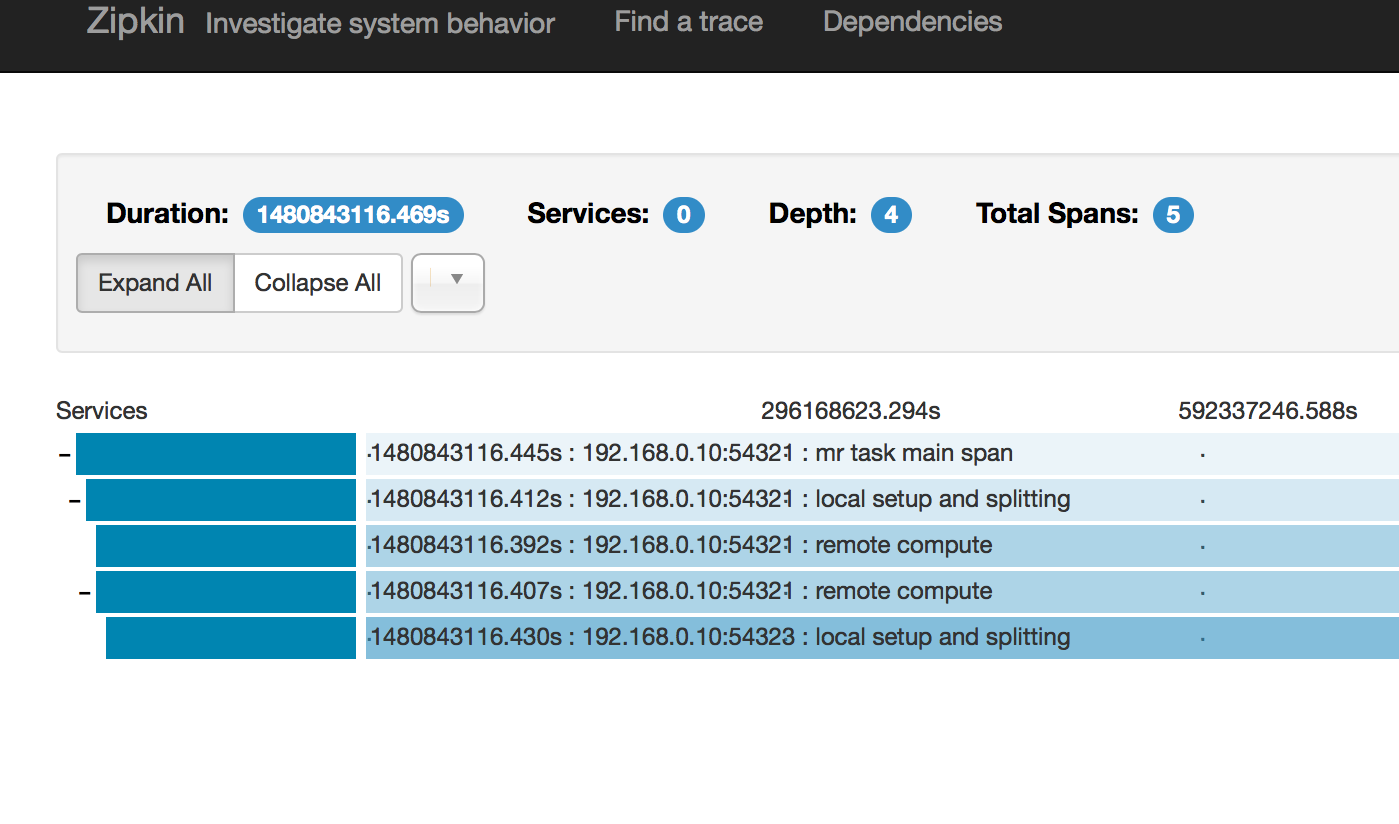
\includegraphics[scale=0.5]{zipkin_ui_example.png}
	\caption{Example of Zipkin UI}
	\label{fig:zipkin_ui}
\end{figure}

Each span in the UI is clickable and all the additional information can bee seen at that level. In this thesis we collect stack trace at each span for monitoring purposes. Example of such information screen can be seen on the figure \ref{fig:zipkin_ui_detail}.
\begin{figure}
	\centering
	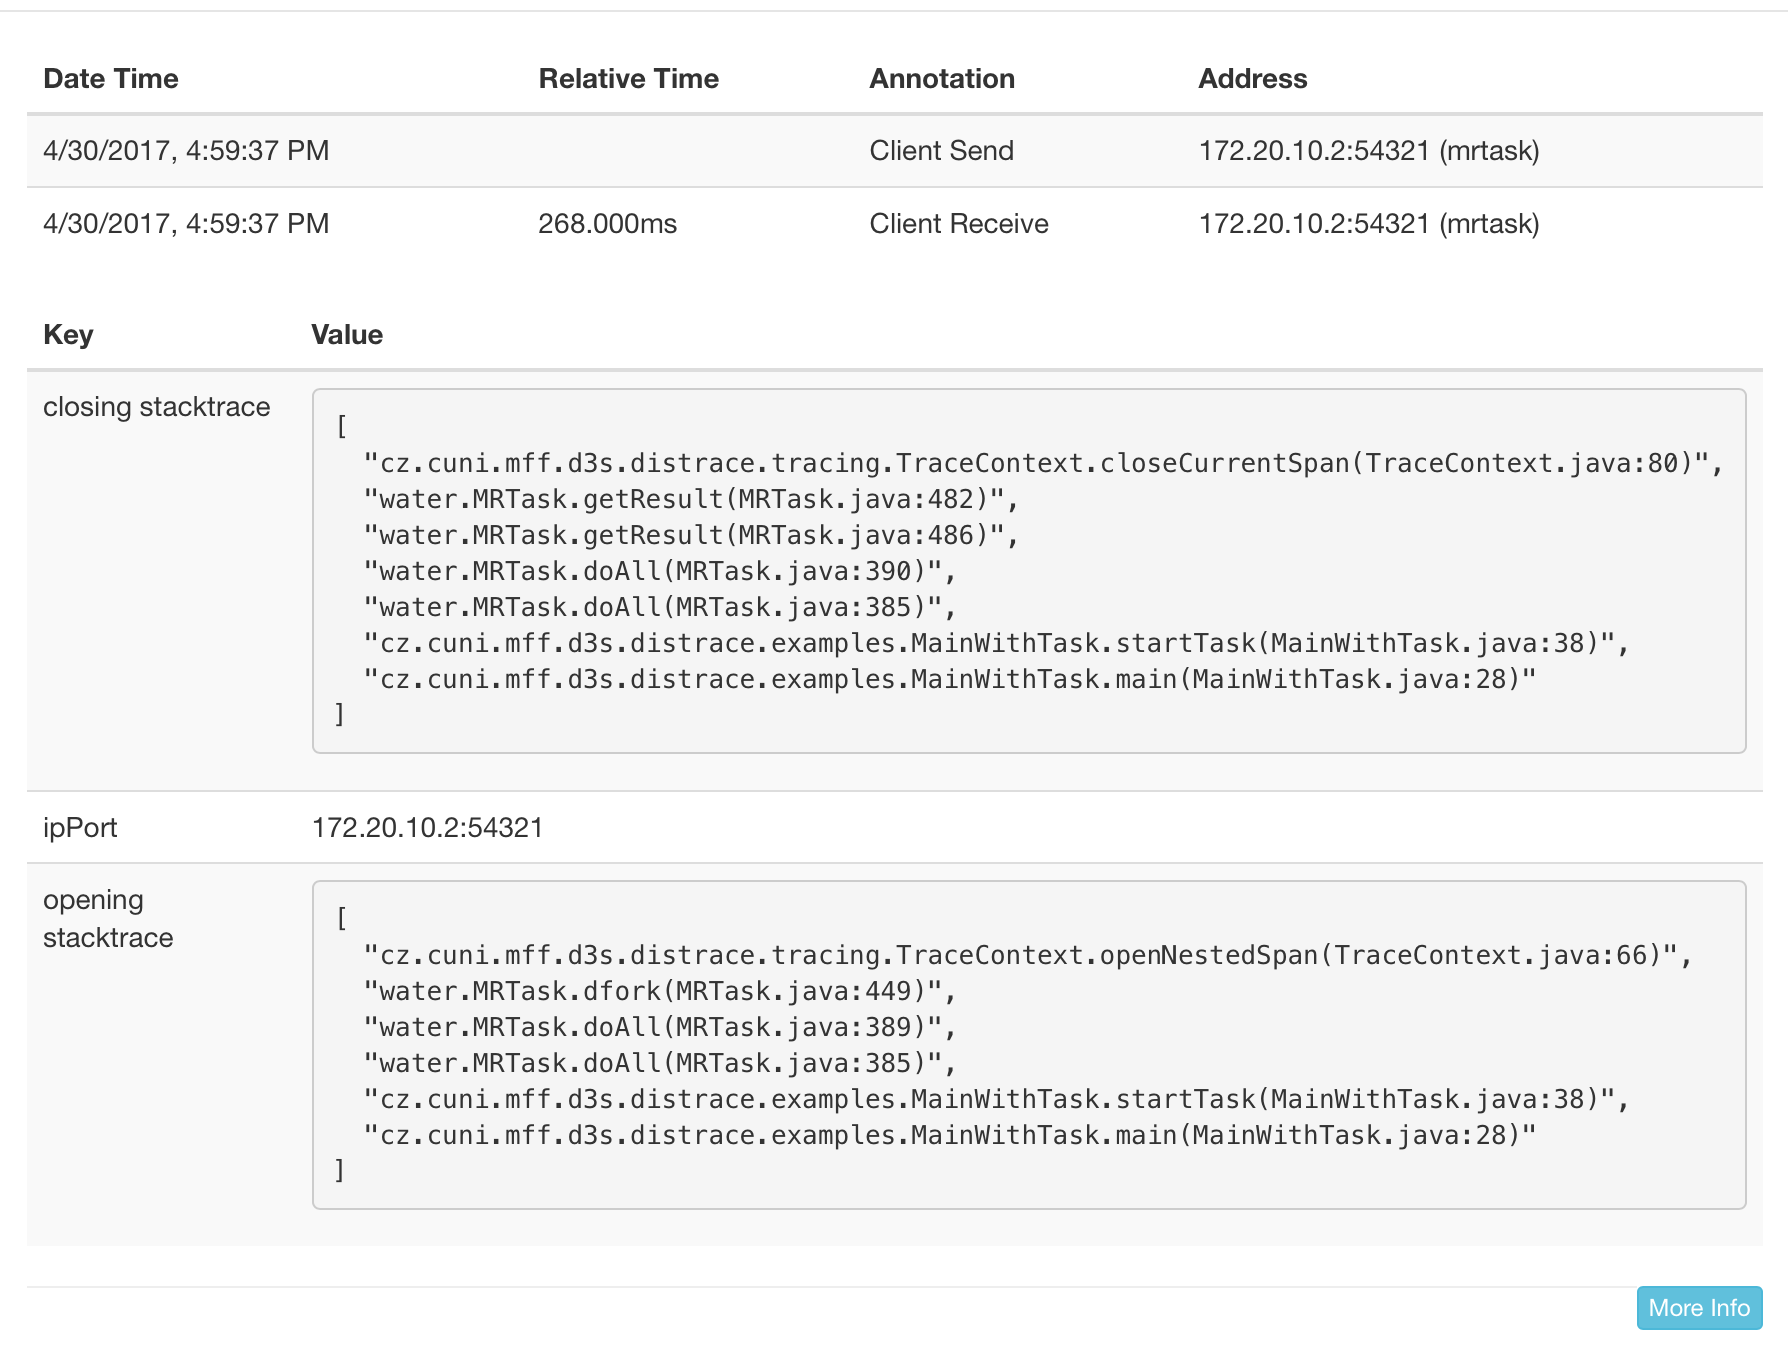
\includegraphics[scale=0.4]{zipkin_ui_detail.png}
	\caption{Example of the detail span information.}
	\label{fig:zipkin_ui_detail}
\end{figure}
\subsection{Zipkin Data Model}
Zipkin requires the data to be sent in JSON format. Requests to UI are sent as JSON arrays where the array elements are the spans them selfs. Zipkin understands the following fields of Span object:
\begin{itemize}
	\item \textbf{traceId} - unique id representing the complete trace. It can be either 128 or 64 bit long.
	\item \textbf{name} - human readable span name
	\item \textbf{id} - id of this span. At the current implementation, Zipkin UI supports span ids only to be 64-bit long.
	\item \textbf{parentId} - parent id of the current span.
	\item \textbf{timestamp} - the time when the span was created.
	\item \textbf{duration} - the duration of the span. It is the time from the creating the span until closing the span.
	\item \textbf{annotations} - array containing standard Zipkin annotations. These annotations can be handled by user interface in specific way since the user interface is understands the meaning of the content. The documentation specifies the following annotations:
	\begin{itemize}
		\item \textbf{cr} : timestamp of client receiving the span
		\item \textbf{cs} : timestamp of client sending the span
		\item \textbf{sr} : timestamp of server reciving the span
		\item \textbf{ss} : timestamp of server receiving the span
		\item \textbf{ca} : client address
		\item \textbf{sa} : server address
	\end{itemize}
	\item \textbf{binaryAnnotations} - array of custom annotations. For example collected stack trace is send as a binary annotation.
\end{itemize}

Except the \textit{annotations} and \textit{binaryAnnotations} fields, the fields are of simple string or number type. Annotations are objects with the 3 fields - annotation value, annotation name and the endpoint. Endpoint is another object specifying the address and port at the code where the span or particular annotation was recorded. Endpoints can also specify service name which may be used to search for particular spans.

Full example of data sent to Zipkin can be:
\begin{lstlisting}[emph={traceId, name, id, timestamp, duration, annotations, value, endpoint, serviceName, ipv4, port, binnaryAnnotations, key},emphstyle={\textbf}]
[
 {
    "traceId": "123456789abcdef",
    "name": "query",
    "id": "abcd1",
    "timestamp": 1458702548467000,
    "duration": 100743,
    "annotations": [
      {
        "timestamp": 1458702548467000,
        "value": "sr"
        "endpoint": {
          "serviceName": "example",
          "ipv4": "192.168.1.2",
          "port": 9411
        },
      }
    ],
    "binaryAnnotations": [
      {
        "key": "bytes_sent",
        "value": "1783"
        "endpoint": {
          "serviceName": "example",
          "ipv4": "192.168.1.2",
          "port": 9411
        },
      }
    ]
 }
]
\end{lstlisting}


